\documentclass[8pt]{article} % use larger type; default would be 10pt

%\usepackage[utf8]{inputenc} % set input encoding (not needed with XeLaTeX)
\usepackage[10pt]{type1ec}          % use only 10pt fonts
\usepackage[T1]{fontenc}
%\usepackage{CJK}
\usepackage{graphicx}
\usepackage{float}
\usepackage{CJKutf8}
\usepackage{subfig}
\usepackage{amsmath}
\usepackage{amsfonts}
\usepackage{hyperref}
\usepackage{enumerate}
\usepackage{enumitem}

\newcommand{\norm}[1]{\left|\left|#1\right|\right|}

%custom commands to save typing
\newcommand{\mynorm}[1]{\left|\left|#1\right|\right|}
\newcommand{\myabs}[1]{\left|#1\right|}

%put subscript under lim and friends
\let\oldlim\lim
\renewcommand{\lim}{\displaystyle\oldlim}
\let\oldmin\min
\renewcommand{\min}{\displaystyle\oldmin}
\let\oldmax\max
\renewcommand{\max}{\displaystyle\oldmax}
\let\oldinf\inf
\renewcommand{\inf}{\displaystyle\oldinf}

\title{Math 1540\\University Mathematics for Financial Studies\\2013-14 Term 1\\Suggested solutions for\\HW problems 12.1}
\begin{document}
\maketitle
\begin{description}
\item[\# 29]{{\it Describe the given sets with a single equation or a pair of equations}
\begin{enumerate}[label=\bfseries\alph*.]
\item{{\it Circle of radius $2$ centered at $(0,2,0)$ and lying in $xy$-plane}. Recall that the intersection of plane and sphere is exactly a circle.
Therefore, we may specify this set just by giving equation of sphere (of radius 2 with centre $(0,2,0)$) and plane. That is
\[
\begin{cases}
(x-0)^2+(y-2)^2+(z-0)^2=4\\z=0
\end{cases}
\]
Of course, the expressions like $x-0$ could be simplified to bare $x$. We write them in this form to facilitate understanding.
}
\item{{\it Circle of radius $2$ centered at $(0,2,0)$ and lying in $yz$-plane.} Similarly to previous example,
\[
\begin{cases}
(x-0)^2+(y-2)^2+(z-0)^2=4\\x=0
\end{cases}
\]}
\item{{\it Circle of radius $2$ centered at $(0,2,0)$ and lying in plane $y=2$.} Similarly to above,
\[
\begin{cases}
(x-0)^2+(y-2)^2+(z-0)^2=4\\y=2
\end{cases}
\]}
\end{enumerate}
\textbf{Note. } It should be kept in mind by students that in this and all subsequent problems that require to describe the given set
of points with equation (or, in general, in any problem, requiring the formula or equation as an answer) the correct answer is \textbf{not unique}! That is, if Your answer is different from that of recommended solution, it is
not the reason to be disappointed or await point deduction. And while answers are better than the others in sense that they
look simpler or more natural, all correct ones shall receive their points.

To promote good style, we shall try to give relatively "good" answers in these solutions, but they are not guaranteed to be the best possible.
In particular, if You think You have a better one, You are welcomed to discuss with TAs.
}
\item[\# 31]{
{\it Describe the given sets with a single equation or a pair of equations}
\begin{enumerate}[label=\bfseries\alph*.]
\item{{\it The line through the point $(1,3,-1)$ parallel to the $x$-axis.} Recall that line may be given as an intersection of two planes (which
may be taken to be mutually perpendicular for simplicity). Now, the plane that would contain this line would have to be either
parallel to $x$-axis, or would have to contain it completely. Also, it should contain point $(1,3,-1)$.

Plane, in turn is fully determined by point it contains and normal vector. As plane should be parallel to $x$-direction, we should find two vectors
that are perpendicular to it to get two planes. $y$- and $z$-directions are natural choices. All this lengthy discussion gives us simple equations
\[\begin{cases}y=3\\z=-1\end{cases}\]

Alternatively, and maybe easily one may observe that the \textit{parametric} equation of this line is apparent, as we are given point and direction:
$(x,y,z)=(1,3,-1)+t\cdot(1,0,0),\;t\in\mathbb{R}$ that can be more readably rewritten as $x=t,\;y=3,\;z=-1$ and clearly gives us two planes we have
been looking for above.
}
\item{{\it The line through the point $(1,3,-1)$ parallel to the $y$-axis.} Similarly to previous example, both geometric and algebraic approach
give us two equation for planes.
\[\begin{cases}x=1\\z=-1\end{cases}\]
}
\item{{\it The line through the point $(1,3,-1)$ parallel to the $z$-axis.} Similarly to above,
\[\begin{cases}x=1\\y=3\end{cases}\]
}
\end{enumerate}
}
\item[\# 33]{{\it Describe the given sets with a single equation or a pair of equations: the circle in which the plane
through the point $(1,1,3)$ perpendicular to $z$-axis meets the sphere of radius $5$ centered at the origin.} As this is often the case, this
problem becomes trivial once You figure out what it asks. Essentially, the set is already given as an intersection of two objects, which naturally
corresponds to system of two equations. The one for sphere is easy, and the one for plane is not much difficult. Plane is determined by normal
vector (vector $(0,0,1)$ is natural representative of $z$-direction) and point it contains: $0\cdot(x-1)+0\cdot(y-1)+1\cdot(z-3)=0$. Coupled with
equation for sphere, this gives us
\[\begin{cases}x^2+y^2+z^2=25\\z=3\end{cases}\]
}
\item[\# 34]{{\it Describe the given sets with a single equation or a pair of equations: the set of points in space that lie $2$ units
from the point $(0,0,1)$ and, at the same time, $2$ units from the point $(0,0,-1)$.} Similarly to problem before this one, we are essentially
given the verbal descriptions of two equations, which we just need to transform to symbols. More precisely, we recall
the formula, hiding behind the word "distance"
\[\begin{cases}\sqrt{x^2+y^2+(z-1)^2}=2\\\sqrt{x^2+y^2+(z-(-1))^2}=2\end{cases}\]

While the above is also a correct answer, it can be simplified. 
Reader equipped with imagination may easily observe, that the intersection of two spheres is a circle (when it has more than one point).
From the badly drawn picture below
\begin{figure}[H]
\centering
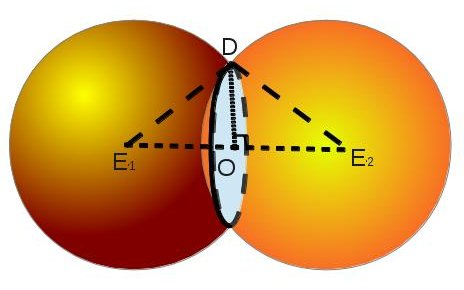
\includegraphics[width=0.6\textwidth]{fin_hw1_spheres}
\end{figure}
it is seen that the center of this circle (indicated as $O$ on a picture) should be located in the middle of the centres of spheres
(indicated as $E_1$ and $E_2$). Therefore, center has coordinates $(0,0,0)$. Consequently, as angle $\angle DOE_2$ is a right angle,
we can apply Pythagorean theorem to $\triangle DOE_2$ to get $DO=\sqrt{DE_2^2-OE_2^2}=\sqrt{3}$. Finally, this circle should lie in a plane that
consists of the points that are equidistant from $E_1$ and $E_2$, that is plane $z=0$. It should be noted that all this information can be derived
not only from the picture, but also from the symmetry considerations: the picture (of two spheres given) is symmetric with respect to reflection
about $z=0$ plane. Anyway, as we know parameters of a circle and a plane containing it, we may readily write an equation describing it, as it
was done in the very first problem of this homework.
Can You derive the 
center, plane containing it and radius? ($(0,0,0)$, $z=0$ and $\sqrt{3}$ respectively) This can be exploited to
 give an alternative answer in the spirit of the first problem of this homework.
\[\begin{cases}x^2+y^2+z^2=3\\z=0\end{cases}\]
}
\item[\# 59]{\begin{enumerate}[label=\bfseries\alph*.]
\item{\textit{Find a formula for the distance from the point $P(x,y,z)$ to the $x$-axis.}
The answer is the most easy to see geometrically, by imagining the plane that contains $x-axis$ and point $P$.
\begin{figure}[H]
\centering
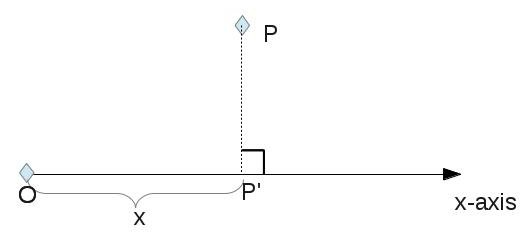
\includegraphics[width=0.6\textwidth]{fin_hw1_linepoint}
\end{figure}
($O$ denotes the origin on a picture, $P'$ is the projection of $P$ on $x$-axis) The distance from point $P$ to $x$-axis is the length of
$PP'$ and that's what we are seeking. As $P'$ is the projection of $P(x,y,z)$ onto $x$-axis, it should have coordinates $P'(x,0,0)$ and therefore
we can apply Pythagorean theorem to the triangle $\triangle OPP'$: $PP'=\sqrt{OP^2-OP'^2}=\sqrt{x^2+y^2+z^2-x^2}=\sqrt{x^2+y^2}$.
}
\item{\textit{Find a formula for the distance from the point $P(x,y,z)$ to the $y$-axis.} Absolutely similar to above,\[D=\sqrt{x^2+z^2}\]}
\item{\textit{Find a formula for the distance from the point $P(x,y,z)$ to the $z$-axis.} Absolutely similar to above,\[D=\sqrt{x^2+y^2}\]}
\end{enumerate}
}
\item[\# 63]{\textit{Find an equation for the set of all points, equidistant from the planes $y=3$ and $y=-1$}. 
	Again, this
is a matter of translating verbal description to formulas, or in particular of using formula for "distance to plane". As planes we are talking
about are both parallel to $xz$-plane and therefore the distance to point $P(x,y,z)$ is computed simply as $D=\myabs{y-3}$ for the plane $y=3$
and $D=\myabs{y-(-1)}$ for $y=-1$.
Now as we are looking for equidistant points we should have
\begin{gather*}
	\myabs{y+1}=\myabs{y-3}\\
	(y+1)^2=(y-3)^2\implies (y+1)^2-(y-3)^2=0\\
	4(2y-2)=0\implies \\y=1
\end{gather*}
}
\item[\# 65]{\begin{enumerate}[label=\bfseries\alph*.]
\item{\textit{Find the point on the sphere $x^2+(y-3)^2+(z+5)^2=4$ nearest to the $xy$-plane. }
	The sphere is of radius 2, centered at  $(0, 3, -5)$, as seen from equation therefore the $z$-coordinate of every point on the sphere lies
	in the interval $[-7,-3]$. As we seek to minimize $\myabs{z}$ (which is exactly the distance to $xy$-plane of an arbitrary point $P(x,y,z)$)
	we will take the point with $z$-coordinate equal to $z=-3$, that is $(0,3,-3)$
	(for substituting $z=-3$ in the equation of sphere gives us $x^2+(y-3)^2+4=4$ and forces $x=y-3=0$)
	that has distance to $xy$-plane equal to \[D=3\]
}
\item{\textit{Find the point on the sphere $x^2+(y-3)^2+(z+5)^2=4$ nearest to the point $(0,7,-5)$. }
	From the picture (given by cross-section with an arbitrary plane passing through $P(0,7,-5)$ and $O(0,3,-5)$)
\begin{figure}[H]
\centering
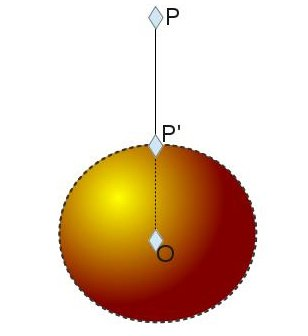
\includegraphics[width=0.6\textwidth]{fin_hw1_pointsphere}
\end{figure}
	it is seen that the closest point to $P(0,7,-5)$ on a sphere is the point $P'$, that lies on intersection of an interval $OP$ and sphere,
	that is point $P'(0,5,-5)$. To make it more precise, note that for an arbitrary $X(x,y,z)$ on the sphere, $XP=
	\sqrt{(x-0)^2+(y-7)^2+(z+5)^2}\geq\myabs{y-7}$. Furthermore, for any $X(x,y,z)$ on the sphere $1\leq y\leq 5$ as may be seen from equation
	of sphere, thus $\myabs{y-7}\geq 2$ and $2$ is exactly the distance $PP'$, so it cannot be surpassed. Anyway, the answer is
	\[D=PP'=2\]
}
\end{enumerate}
}
\item[\# 66]{To begin with, we note that the set of points, equidistant from two points, form a plane and therefore the point we are looking for
lies on intersection of planes. To see the fact claimed, simple derivation is enough: assume we are looking for the simple equation describing the 
set of points, equidistant from $P(x_0,y_0,z_0)$ and $M(x_1,y_1,z_1)$
\begin{gather*}
\sqrt{(x-x_0)^2+(y-y_0)^2+(z-z_0)^2}=
\sqrt{(x-x_1)^2+(y-y_1)^2+(z-z_1)^2}\\
(x-x_0)^2+(y-y_0)^2+(z-z_0)^2=
(x-x_1)^2+(y-y_1)^2+(z-z_1)^2\\
\left((x-x_0)^2-(x-x_1)^2\right)+
\left((y-y_0)^2-(y-y_1)^2\right)+
\left((z-z_0)^2-(z-z_1)^2\right)=0\\
\left((x-x_0)-(x-x_1)\right)\left((x-x_0)+(x-x_1)\right)+
\left((y-y_0)-(y-y_1)\right)\left((y-y_0)+(y-y_1)\right)+\\
+\left((z-z_0)-(z-z_1)\right)\left((z-z_0)+(z-z_1)\right)=0\\
(x_1-x_0)(2x-x_0-x_1)+
(y_1-y_0)(2y-y_0-y_1)+
(z_1-z_0)(2z-z_0-z_1)=0\\
2(x_1-x_0)\cdot x+
2(y_1-y_0)\cdot y+
2(z_1-z_0)\cdot z=\\=
(x_1-x_0)(x_0+x_1)+
(y_1-y_0)(y_0+y_1)+
(z_1-z_0)(z_0+z_1)
\end{gather*}
the last equation is just an equation of a plain.

Now, we may derive three planes from the given set of 4 points. Applying the formula above, we see that 
\begin{itemize}
\item{Points, equidistant from $(0,0,0)$ and $(0,4,0)$ form a plane \[y=2\]}
\item{Points, equidistant from $(0,0,0)$ and $(3,0,0)$ form a plane \[x=1.5\]}
\item{Points, equidistant from $(0,0,0)$ and $(2,2,-3)$ form a plane \[4x+4y-6z=17\]}
\end{itemize}

As the point we are looking for lies on all of the planes mentioned above, it is easily seen to be
\[x=1.5,\;y=2,\;z=-0.5\]
}
\end{description}
\end{document}
